\documentclass[9pt]{extarticle}
\usepackage{blindtext}
\usepackage{amsmath}
\usepackage[parfill]{parskip}

\title{Cutting plane algorithm: \\ an interactive web application}
\date{October 2020}
\author{Riccardo Locci}

\usepackage{algorithm}
\usepackage[noend]{algpseudocode}

\makeatletter
\def\BState{\State\hskip-\ALG@thistlm}
\makeatother

\usepackage{listings}
\usepackage{xcolor}

\newcommand\JSONNumberValueStyle{\color{olive}}
\newcommand\JSONStringValueStyle{\color{orange}}
\newcommand\JSONStringKeyStyle{\color{purple}}

% switch used as state variable
\newif\ifcolonfoundonthisline

\makeatletter

    \lstdefinestyle{json}
    {
        showstringspaces    = false,
        keywords            = {false,true},
        alsoletter          = 0123456789.,
        morestring          = [s]{"}{"},
        stringstyle         = \ifcolonfoundonthisline\JSONStringValueStyle\else\JSONStringKeyStyle\fi,
        MoreSelectCharTable =%
            \lst@DefSaveDef{`:}\colon@json{\processColon@json},
        basicstyle          = \ttfamily,
        keywordstyle        = \ttfamily\bfseries,
        gobble              = 12,
        numbers=left, stepnumber=1, numberstyle=\small, numbersep=10pt
    }

    % flip the switch if a colon is found in Pmode
    \newcommand\processColon@json{%
    \colon@json%
    \ifnum\lst@mode=\lst@Pmode%
        \global\colonfoundonthislinetrue%
    \fi
    }

    \lst@AddToHook{Output}{%
    \ifcolonfoundonthisline%
        \ifnum\lst@mode=\lst@Pmode%
        \def\lst@thestyle{\JSONNumberValueStyle}%
        \fi
    \fi
    %override by keyword style if a keyword is detected!
    \lsthk@DetectKeywords% 
    }

    % reset the switch at the end of line
    \lst@AddToHook{EOL}%
    {\global\colonfoundonthislinefalse}

\makeatother

\usepackage{graphicx}
\graphicspath{ {./images/} }

\usepackage[hidelinks]{hyperref}
\usepackage{amsfonts}

\usepackage{mathtools}
\DeclarePairedDelimiter\ceil{\lceil}{\rceil}
\DeclarePairedDelimiter\floor{\lfloor}{\rfloor}

\algdef{SE}{Begin}{End}{\textbf{begin}}{\textbf{end}}

\begin{document}
    \maketitle
        
    \begin{abstract} 
        In mathematical optimization, the cutting-plane method is any of a variety of optimization methods that iteratively 
        refine a feasible set or objective function by means of linear inequalities, termed cuts. 
        Such procedures are commonly used to find integer solutions to mixed integer linear programming (MILP) problems, 
        as well as to solve general, not necessarily differentiable convex optimization problems. The use of cutting planes 
        to solve MILP was introduced by Ralph E. Gomory.\cite{wiki:cuttingplane} 

        Focus of this work is to propose the implementation of the cutting plane algorithm as an interactive web application
        that shows the algorithm's execution flow step-by-step.
        This work will result in a auxiliary learning tool to better understand and visualize how the algorithm works
        thanks to the grafical user interface exposed by the application.
        Since the developed application focuses on a geometric representation of the algorithm, it is thought to work
        with two decisional variables.
        The application was develop and tested on Google Chrome on the following machines:
        
        \begin{itemize}
            \item Desktop:
            \begin{itemize} 
                \item OS: Windows 10 Pro 1903, 
                \item CPU: Intel\textregistered Core i5-4440 3.10 GHz
                \item RAM: 16 GB DDR3 
            \end{itemize}
            \item MacBook Air:
            \begin{itemize} 
                \item OS: macOS Catalina 10.15.5, 
                \item CPU: Intel\textregistered Core i5 dual-core 1.6 GHz
                \item RAM: 8 GB LPDDR3 
            \end{itemize}
        \end{itemize}
    \end{abstract}

    \begin{section}{Integer Linear Programming formal definition}

        Linear programming (LP, also called linear optimization) is a method to achieve the best outcome (such as maximum 
        profit or lowest cost) in a mathematical model whose requirements are represented by linear relationships.
        \cite{wiki:lp}

        More formally, linear programming is a technique for the optimization of a linear objective function, subject to 
        linear equality and linear inequality constraints. 
        Its feasible region is a convex polytope, which is a set defined as the intersection of finitely many half spaces, 
        each of which is defined by a linear inequality. 
        Its objective function is a real-valued affine (linear) function defined on this polyhedron. 
        A linear programming algorithm finds a point in the polytope where this function has the smallest (or largest) 
        value if such a point exists. \cite{wiki:lp}
        \newpage

        Linear programs are problems that can be expressed in canonical form as:
        
        \begin{equation*}
            \begin{array}{ll@{}ll}
                \text{maximize}  & c^{T}x \\
                \text{subject to} & Ax \leq b \\
                \text{and} & x \ge 0
            \end{array}
        \end{equation*}

        where $x$ represents the vector of variables (to be determined), $c$ and $b$ are vectors of (known) coefficients and 
        $A$ is a (known) matrix of coefficients.
        The expression to be maximized or minimized is called the objective function ($c^{T}x$ in this case). 
        The inequalities $Ax \leq b$ and $x \ge 0$ are the constraints which specify a convex polytope over which the objective 
        function is to be optimized. 
        In this context, two vectors are comparable when they have the same dimensions. 
        If every entry in the first is less-than or equal-to the corresponding entry in the second, then it can be said 
        that the first vector is less-than or equal-to the second vector.
        \cite{wiki:lp}

        Linear programming can be applied to various fields of study. 
        It is widely used in mathematics, and to a lesser extent in business, economics, and for some engineering problems. 
        Industries that use linear programming models include transportation, energy, telecommunications, and manufacturing. 
        It has proven useful in modeling diverse types of problems in planning, routing, scheduling, assignment, and design.
        \cite{wiki:lp}

        An integer programming problem is a mathematical optimization or feasibility program in which some or all of the 
        variables are restricted to be integers. 
        In many settings the term refers to integer linear programming (ILP), in which the objective function and the 
        constraints (other than the integer constraints) are linear.

        An integer linear program in canonical form is expressed as:

        \begin{equation*}
            \begin{array}{ll@{}ll}
                \text{maximize}  & c^{T}x \\
                \text{subject to}& Ax \leq b \\
                \text{and} & x \ge 0 \\
                \text{and} & x \in \mathbb{Z}^n \\
            \end{array}
        \end{equation*}

    \end{section}

    \begin{section}{Overview about Cutting Plane Method}
        Cutting plane methods for MILP work by solving a non-integer linear program, the linear relaxation of the given integer 
        program. 
        The theory of Linear Programming dictates that under mild assumptions (if the linear program has an optimal solution, 
        and if the feasible region does not contain a line), one can always find an extreme point or a corner point that is 
        optimal. 
        The obtained optimum is tested for being an integer solution. 
        If it is not, there is guaranteed to exist a linear inequality that separates the optimum from the convex hull of the 
        true feasible set. 
        Finding such an inequality is the separation problem, and such an inequality is a cut. 
        A cut can be added to the relaxed linear program. Then, the current non-integer solution is no longer feasible to the 
        relaxation. 
        This process is repeated until an optimal integer solution is found. \cite{wiki:cuttingplane}
        
        \begin{subsection}{Algorithm}
            The method proceeds by first dropping the requirement that the $x_i$ be integers and solving the associated linear 
            programming problem to obtain a basic feasible solution. 
            Geometrically, this solution will be a vertex of the convex polytope consisting of all feasible points. 
            If this vertex is not an integer point then the method finds a hyperplane with the vertex on one side and all 
            feasible integer points on the other. 
            This is then added as an additional linear constraint to exclude the vertex found, creating a modified linear 
            program. 
            The new program is then solved and the process is repeated until an integer solution is found.
            \cite{wiki:cuttingplane}

            Using the simplex method to solve a linear program produces a set of equations of the form:
            \begin{equation*}
                x_i + \sum{\overline{a}_{ij}x_j} = \overline{b}_i
            \end{equation*}

            where $x_i$ is a basic variable and the $x_j$'s are the nonbasic variables. 
            Rewrite this equation so that the integer parts are on the left side and the fractional parts are on the right side:
            \begin{equation*}
                x_i + \sum{
                    \floor*{
                        \overline{a}_{ij}}
                    }x_j - \floor*{
                        \overline{b}_i
                     } = \overline{b}_i - \floor*{
                        \overline{b}_i
                     } - \sum{
                         (\overline{a}_{ij} - \floor*{
                            \overline{a}_{ij}
                        })x_j
                     }
            \end{equation*}

            For any integer point in the feasible region the right side of this equation is less than 1 and the left side is 
            an integer, therefore the common value must be less than or equal to 0. 
            So the inequality:
            \begin{equation*}
                \overline{b}_i - \floor*{
                        \overline{b}_i
                     } - \sum{
                         (\overline{a}_{ij} - \floor*{
                            \overline{a}_{ij}
                        })x_j
                     } \leq 0
            \end{equation*}

            must hold for any integer point in the feasible region. 
            Furthermore, nonbasic variables are equal to 0s in any basic solution and if $x_i$ is not an integer for the basic 
            solution $x$,
            \begin{equation*}
                \overline{b}_i - \floor*{
                        \overline{b}_i
                     } - \sum{
                         (\overline{a}_{ij} - \floor*{
                            \overline{a}_{ij}
                        })x_j
                     } = \overline{b}_i - \floor*{
                        \overline{b}_i
                     } > 0
            \end{equation*}

            So the inequality above excludes the basic feasible solution and thus is a cut with the desired properties. 
            Introducing a new slack variable $x_k$ for this inequality, a new constraint is added to the linear program, namely:
            \begin{equation*}
                x_k + \sum{
                    (\overline{a}_{ij} - \floor*{
                        \overline{a}_{ij}
                    })x_j = \floor*{
                        \overline{b}_i
                     } - \overline{b}_i,\ x_k \ge 0,\ x_k \ \text{an integer}
                }
            \end{equation*}
        \end{subsection}

        \begin{subsection}{Pseudocode}
            The following pseudocode\cite{book} represents the classical version of the algorithm, which will be used as a kickstart
            for the final web application:
            \vspace{10px}

            \begin{algorithm}
                \caption{Cutting Plane Algorithm}\label{alg:cuttingplane}
                \begin{algorithmic}[1]
                    \Procedure{Cutting Plane}{}
                        \State \parbox[t]{.8\linewidth}{%
                            solve the continuous relaxation 
                            $\min\{\mathbf{c}^{T}\mathbf{x} : \text{A}\mathbf{x} = \mathbf{b}, \mathbf{x} \ge 0\}$
                            and let $\mathbf{x^*}$ be the basic optimal solution found
                        }
                        \While {$\mathbf{x^*}$ not integer}
                            \State \parbox[t]{.8\linewidth}{%
                                solve the separation problem of $\mathbf{x^*}$ from $X$ by finding an inequality
                                $\alpha^{T}\mathbf{x} \leq \alpha_0$ valid for $X$ but violated by $\mathbf{x^*}$
                            }
                            \State add the constraint $\alpha^{T}\mathbf{x} \leq \alpha_0$ to the current continuous relaxation
                            \State \parbox[t]{.8\linewidth}{%
                                solve current continuous relaxation (through dual simplex algorithm) and let $\mathbf{x^*}$ 
                                be the new basic optimal solution found
                            }
                        \EndWhile
                    \EndProcedure
                \end{algorithmic}   
            \end{algorithm}    
            \vspace{10px}     
        \end{subsection}
    \end{section}

    \begin{section}{Implementation of the algorithm}
        In this section we will discuss the proposed implementation, but first there are some aspects that require some 
        clarifications. 
        All the problems solvable through the implementation need to be limited to two decisional variable, since the focus of
        the work is to show a geometrical representation of how the method proceeds to find a solution.
        Another point of discussion will be the algorithm itself: to allow the application to behave in the right way, 
        \textbf{Algorithm \ref{alg:cuttingplane}} will be split in multiple steps. \\
        Finally, since the target of this work is to create a graphical user interface to illustrate and better understand
        cutting-plane algorithm, computational complexity was not taken into account: this obviously leaves space for future 
        optimizations.

        \begin{subsection}{Data structures}
            The application uses a set of matrices to store the values computed at each step of the method.
            The same matrices are then used to assemble the tableau representation of the problem, which is shown on the graphical 
            user interface.
            Considering that the target of this work was to implement cutting-plane algorithm, the drawing effort was delegated to
            a ready-to-use library\cite{github:plotly} to cut development times.

            A sample problem is then represented by the following JSON file:

            \vspace{10px}
            \begin{lstlisting}[style=json,caption={JSON file example},captionpos=b,label={data:json}]
                {
                    "variables": ["x1", "x2"],
                    "objectiveFunction": [0, -1],
                    "subjectTo": {
                        "A": [
                            [3, 2],
                            [-3, 2]
                        ],
                        "b": [6, 0],
                        "sign": [-1, -1]
                    }
                }
            \end{lstlisting}
            \vspace{20px}
            
            The result will be the following (starting) geometrical representation:
            \vspace{10px}
            \begin{figure}[h]
                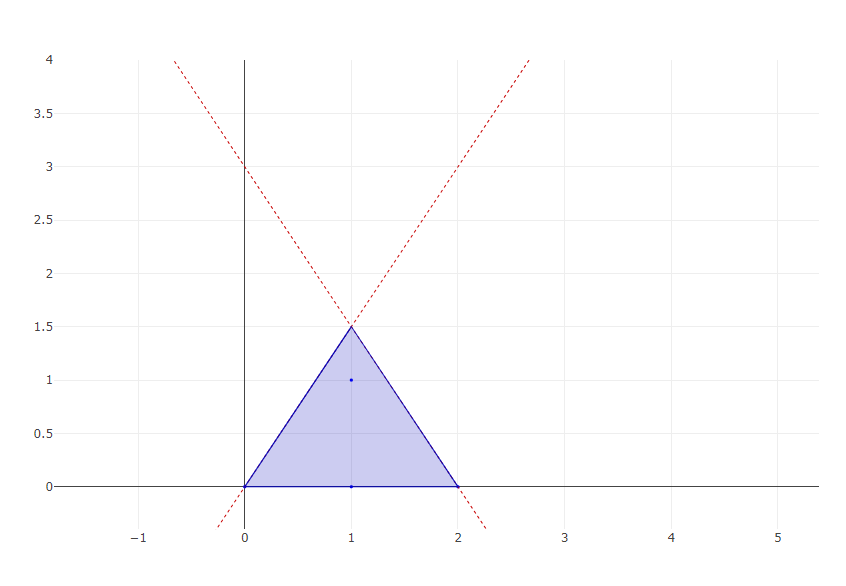
\includegraphics[scale=0.4]{problem1.png}
                \centering
                \vspace{20px}
                \begin{description}
                    \centering
                    \item[Figure 1] Admissible plane drawn from Listing \ref{data:json}
                \end{description}
            \end{figure}
            \vspace{10px}
            
            The separation of the matrices allows a better representation of the tableau (each section can be highlighted as one
            wishes) and simplifies operations between different parts.
            Since the project was written using JavaScript programming language, some problems rise up with error propagation due to
            the numerical representation: in this sense, an external library was used for linear algebra operations \cite{github:numbers}. 
            
            Additional lists are then used to keep track of the geometrical representation.
            We have:
            \begin{itemize}
                \item a list of points, that determines the polygon being drawn;
                \item a list of points, that stores the admissible integer points within the polygon;
                \item a list of lines, that is used to draw the constraints of the problem.
            \end{itemize}
        \end{subsection}
        
        \begin{subsection}{Custom implementation}
            The classical implementation of the cutting-plane algorithm work as a unique flow that from an input graph computes shortest paths 
            and returns them as their output.
            This work will obviously return the same output of a classical implementation, but it will also show every step that
            leads to the computation of every intermediate solution.
            It follows that the algorithm cannot work as a single block of code, but it needs to be split and modularized in multiple phases.

            The following sections will cover the content of the three phases of the custom algorithm.

            \begin{subsubsection}{Admissible space computation}
                The drawing of the starting admissible space is the first operation that will run after input is provided. 
                Its role is to populate the supporting data structures and initialize other data structures used by other features 
                (i.e.: navigable algorithm's history).
                It starts from a finite square that covers the positive section of the cartesian plane for both the variables, and intersects it
                by the portion of plane defined by the constraints to obtain the continuous admissible plane.
                The integer admissible space is then obtained by highlighting the points with integer coordinates that are contained within the
                drawn polyhedron.
                Everytime a new cut is found, this procedure is run, so that at every step of the algorithm the geoemtrical representation is
                up-to-date.
            \end{subsubsection}

            \begin{subsubsection}{Continuous optimal solution}
                The first phase takes care of finding the optimal solution of the contiuous relaxation of the problem through the resolution of
                the simplex algorithm \cite{wiki:simplex}, in its tableau form.
                This phase covers the first instruction of \textbf{Algorithm \ref{alg:cuttingplane}}.
                At each step, the algorithm selects a basic variable and a nonbasic variable and switches them to improve the value of the 
                objective function.
                Each pair of variable selected determines a pivot element, that is then used to update every row of the tableau to keep its feasibility.
                The algorithm stops when it cannot select a nonbasic variable whose entrance in the base would improve the value of the objective
                function, or the solution found is not feasible.
                If the algorithm successfully stops, we have a valid optimal solution that can be used to find a valid integer optimal solution. 
            \end{subsubsection}

            \begin{subsubsection}{Integrality check and cut search}
                The previously found solution needs to pass an integrality check to be declared as optimal for the integer problem.
                If all the components of the current solution are integer, then we already have solved the problem.
                Conversely, we need to find a cut that invalidates the previous solution while keeping the admissible integer solutions.
                Practically speaking, we introduce a new slack variable for the cut found and a constraint to the previous problem,
                obtaining a new linear programming problem that can be solved in the next step.
            \end{subsubsection}

            \begin{subsubsection}{New continuous relaxation resolution}
                Every time a new cut is found, and a new contraint is added to the previous relaxation problem, the new problem needs to be solved
                through the dual simplex method.
                While classic simplex tries to find a nonbasic variable whose entrance in the base will improve the value of the objective function,
                the dual version works by finding a good basic variable that will leave the base.
                The pair of selected variables will again identify a pivot element that is the used to update the rows of the current tableau.
                Once the dual algorithm finishes, we have a solution that needs again to be tested for integrality.
            \end{subsubsection}
        \end{subsection}

        \begin{subsection}{Web application GUI}
            Within this section we will show how the application appears and which parts compose the Graphical User Iterface:
            we will talk about all the possible interactions and features, and how they influence the understanding of the 
            algorithm.
            
            \begin{figure}[h]
                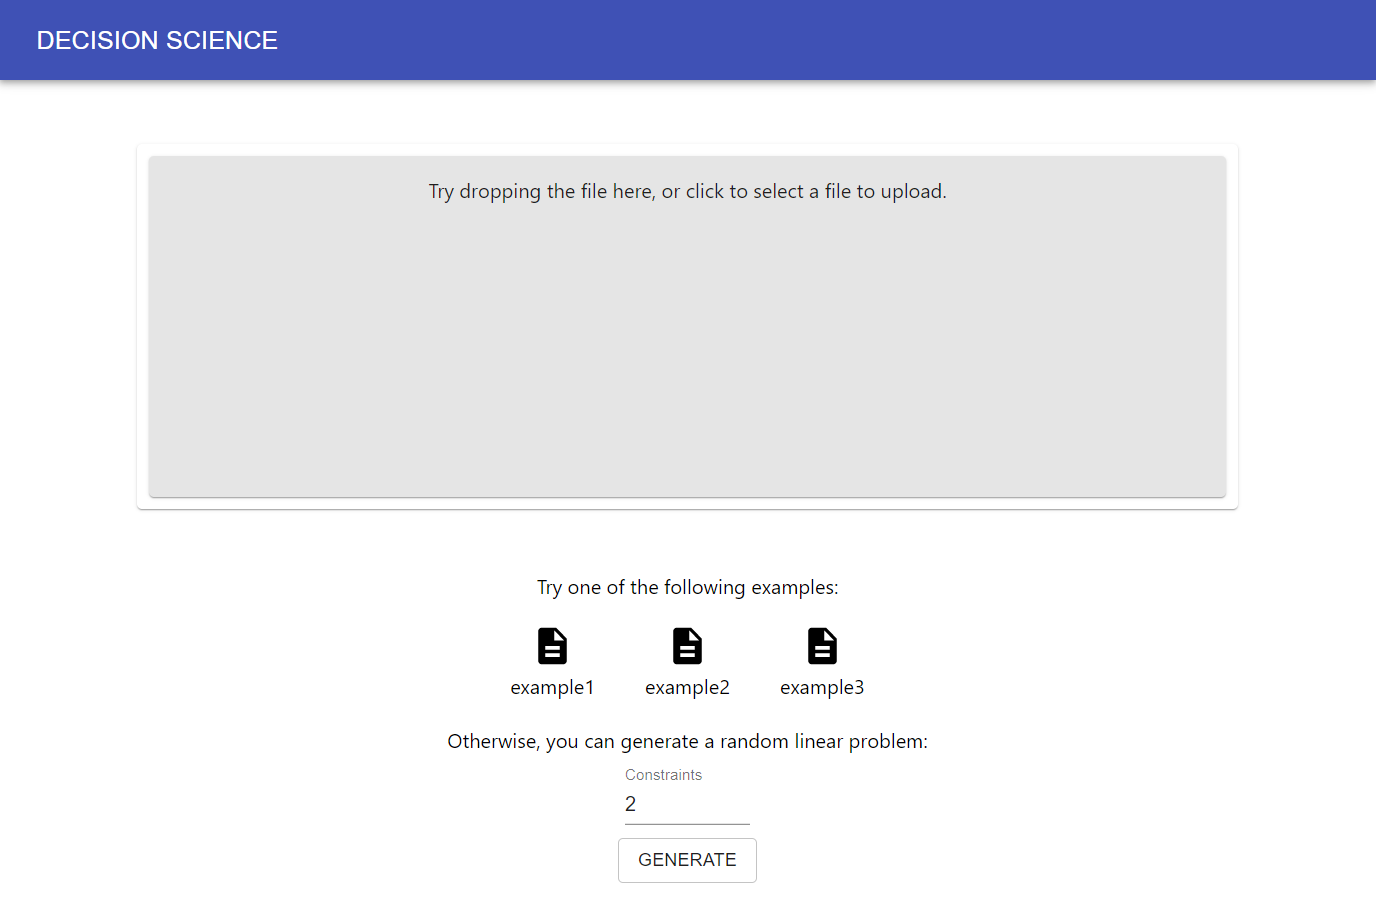
\includegraphics[scale=0.23]{gui1.png}
                \centering
                \begin{description}
                    \centering
                    \item[Figure 2] Landing page and input choice 
                \end{description}
            \end{figure}

            \begin{subsubsection}{Input choices}
                \label{subsec:input}
                First page of the web application\cite{web:app} allows multiple ways to provide a problem as input for the algorithm. 
                The page is divided in three sections:
                
                \begin{itemize}
                    \item a \textbf{drop area} where to drop a properly formatted JSON file describing a problem (see Listing \ref{data:json}): 
                            it is also possible to select a file from file explorer by clicking over the area;
                    \item a small set of \textbf{sample problems} on which the application was tested: every file presents a name that points the 
                            number of nodes and arcs;
                    \item a \textbf{generation form} that allows the user to create a pseudo-random linear programming problem with two decisional
                            variables.
                \end{itemize}

                The generation form only needs the number of constraints that the problem will contain.
                The maximum number of constraints is limited to 50 since a greater number would be chaotic on the geometrical representation.
            \end{subsubsection}

            \begin{subsubsection}{Geometric representation}
                After input is provided, the graph will be drawn in the canvas: its purpouse is to help understanding what is happening while the 
                algorithm runs.
                In this section we can see the polygon created by the constraints (admissible space of the continuous relaxation) and each one of the 
                points with integer coordinates (admissible solutions of the integer problem).
                At each step, the current solution is identified by a green point to better understand how it changes during the execution of the
                algorithm.
                Every contraint is defined by a red dotted line, and each one identifies a half-plane that contributes to show the admissible space
                of the continuous relaxation.
            \end{subsubsection}
            
            \begin{figure}[h]
                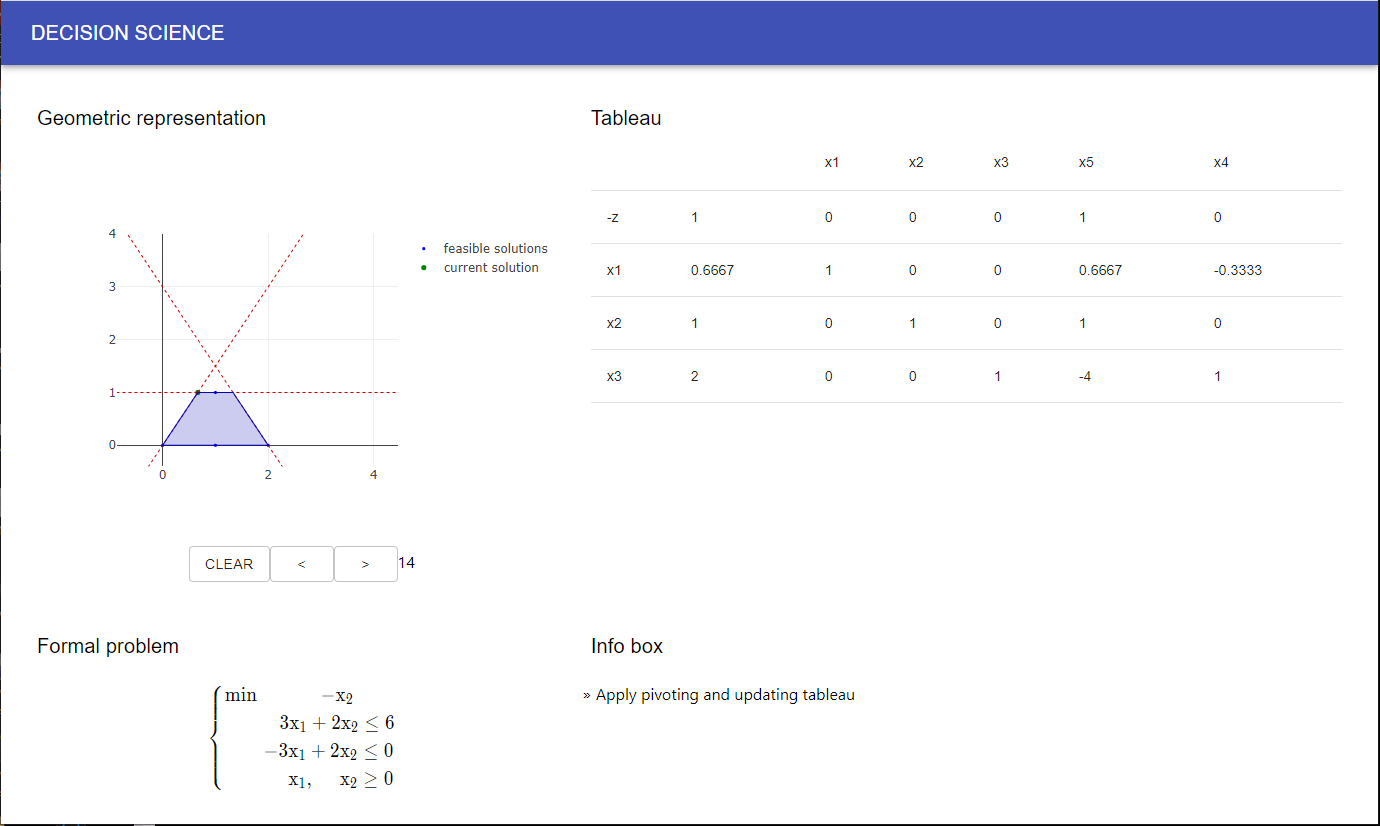
\includegraphics[scale=0.3]{gui2.png}
                \centering
                \begin{description}
                    \centering
                    \item[Figure 4] Application GUI example
                \end{description}
            \end{figure}

            \begin{subsubsection}{Tableau}
                On the top right section, during the execution of the algorithm, a tableau representation will be shown.
                It keeps track of the various data structures used within this implementation such as:
                \begin{itemize}
                    \item the negative of the current value of the objective function;
                    \item the current costs of the basic variables;
                    \item the current costs of the nonbasic variables;
                    \item the current value of the basic variables;
                    \item the current value of the coefficients of basic variables;
                    \item the current value of the coefficients of nonbasic variables;
                \end{itemize}
                
                To not be excessively verbose, not all the changes on the tableau are reflected by the graphical user iterface, for example
                the pivoting operation is not completely shown: at each step the GUI can show the column gave by the entering nonbasic variable,
                the row gave by the leaving basic variable (if both are highlighted, the pivot value is highlighted too), and the new tableau obtained
                after the pivoting operation.
            \end{subsubsection}

            \begin{subsubsection}{Interaction section}
                \label{subsec:interaction}

                Below the canvas there are some elements that help to iteract with the application:
                \begin{itemize}
                    \item the \textbf{clear button} reverts the current state of the application and sends the user back to the input page;
                    \item the \textbf{download button} allows to download the current drawn graph as a JSON file;
                    \item the \textbf{navigation buttons} are used to keep executing the algorithm and visualize its history.
                \end{itemize}

                Every time the algorithm has to keep executing, the user need to press on the \textbf{Next} button (the navigation button on the 
                right): the new state is computed only once then it is stored within a proper data structure. 
                By storing every state, the application allows to navigate algorithm execution history back and forth.

            \end{subsubsection}

            \begin{subsubsection}{Formal problem representation}
                Bottom left section is dedicated to show the starting problem in canonical form. 
                To draw this part of the GUI was used a external library that parses a LaTeX document.
                The LaTeX document is computed right after the input is provided, and it is not changed by the application during algorithm execution.
            \end{subsubsection}

            \begin{subsubsection}{Info box}
                The last section provides written descriptions of what it is happening in a given state of the algorithm.
                Every step produces a change in almost all the section of the graphical user interface (except for the formal problem representation 
                section, that only shows the starting problem), which is intuitevely understandable thanks to its graphical and geometrical nature; 
                however, there are steps that cannot be effectively communicated through figures and need a written explanation.
            \end{subsubsection}
        \end{subsection}
    \end{section}

    \begin{section}{Results and performances}
        This application can successfully run a (properly customized) classical implementation of cutting-plane algorithm for integer linear 
        programming problems. 
        It was tested on a set of problems provided within the \textbf{book}\cite{book} and on \textbf{IBM ILOG CPLEX Optimization Studio}
        \cite{web:cplex}: to compare the results a Python script (see GitHub repository \cite{github:project}) was developed to convert JSON files 
        to CPLEX models and then the resulting objective functions were compared. 
        All the tests returned the same results on both the web application and IBM ILOG CPLEX Optimization Studio.

        The application does not allow to jump to the end of the execution since its objective is to illustrate how the algorithm behaves at every 
        step, so its performaces were not taken into account (multiple matrixes instead of a unique one containing the tableau). 
        Since the objective of the work was to show the progression of the algorithm from a geometrical point of view, besides the support section
        added (info box, tableau representation, etc.), the problems solved were limited to two decisional variables (obviously limiting their 
        complexity), so the principal challange to the performaces was only given by the number of contraints on a given problem (that potentially 
        increases during the execution): due to this limits, this work did not show any particular performances' issue.
    \end{section}

    \begin{section}{Conclusions}
        The developed web application described in this work allows to correctly run cutting-plane algorithm on problems provided as JSON files 
        or generated through the application's generator, and to see a step-by-step execution thanks to a user-friendly interface that at each 
        iteration draws a geometrical representation and describes what it is really happening from the beginning to the end. 
        Moreover it is possible not only to proceed forward into the execution, but to go back in time, too: this feature allows a better 
        understanding and analysis of the algorithm and provides a different perspective.

        At this point in development, the application is surely useful when studying cutting-plane algorithm, but there are many optimizations
        and features that can be considered to improve this work. 
        An optimized algorithm to generate the polygon that defines the admissible space, a better organization of the interface to improve 
        user experience, multiple algorithms to choose, support for other input formats (e.g.: direct support for CPLEX models): this are just 
        some example of how the application can be extended in the future.
    \end{section}

    \begin{thebibliography}{7}

        \bibitem{wiki:cuttingplane} 
        Wikipedia,
        \textit{Cutting plane algorithm},
        \url{https://en.wikipedia.org/wiki/Cutting-plane_method}

        \bibitem{wiki:lp} 
        Wikipedia,
        \textit{Linear programming},
        \url{https://en.wikipedia.org/wiki/Linear_programming}

        \bibitem{book} 
        Matteo Fischetti
        \textit{ Lezioni di Ricerca Operativa }

        \bibitem{github:plotly} 
        GitHub,
        \textit{React Plotly}:
        \url{https://github.com/plotly/react-plotly.js/}

        \bibitem{github:numbers} 
        GitHub,
        \textit{Numbers.js}:
        \url{https://github.com/numbers/numbers.js/}

        \bibitem{wiki:simplex} 
        Wikipedia,
        \textit{Simplex algorithm},
        \url{https://en.wikipedia.org/wiki/Simplex_algorithm}

        \bibitem{web:app} 
        Project Web Application: \url{https://riccardolocci.github.io/DS}
        
        \bibitem{web:cplex} 
        CPLEX,
        \textit{IBM ILOG CPLEX Optimization Studio},
        \url{https://www.ibm.com/it-it/products/ilog-cplex-optimization-studio}

        \bibitem{github:project} 
        GitHub,
        \textit{Project Repository},
        \url{https://github.com/riccardolocci/DS}

    \end{thebibliography}

\end{document}